% !TEX encoding = UTF-8 Unicode
% !TEX TS-program = pdflatex
 \documentclass[%
 	12pt,
 	a4paper
]{article}
%%%%%%%%%%%%%%%%%%%%%%%%%%%%%%%%%%%%%%%%%%%%%%%%%%%%
\usepackage[utf8]{inputenc}
\usepackage[T1]{fontenc}
\usepackage[british, italian]{babel}
\usepackage{lmodern}
\usepackage{amsmath}
\usepackage{amssymb}
\usepackage{amsthm}
\usepackage{xspace}% per i colori
\usepackage{graphicx}
\usepackage{emptypage} % pagina tutta bianca a fine capitolo
\usepackage{pdfpages} % per inserire pdf
\PassOptionsToPackage{hyphens}{url}
\usepackage{hyperref} % va caricato per ultimo
\hypersetup{%
	pdfpagemode={UseOutlines},
	bookmarksopen,
	pdfstartview={FitH},
	hidelinks
}
\pdfminorversion=7 % per togliere il warning delle immagini
\pagenumbering{gobble}
\begin{document}
%\begin{figure}
%	\centering
%	\includegraphics[
%	trim={1cm 16.7cm 11cm 10.5cm}, clip]{logo.pdf}
%\end{figure}
\begin{figure}
	\centering
	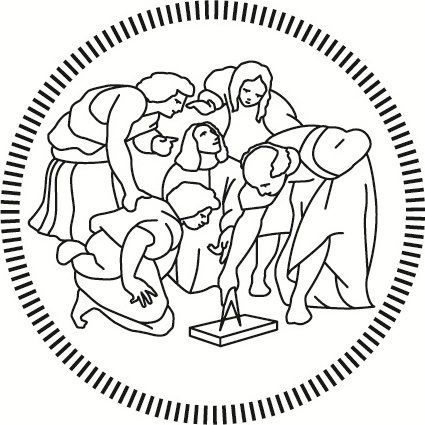
\includegraphics[width=2.5cm]{../../img/logopoli.png}\\
	\caption{png}
	
\includegraphics[width=2.5cm]{../../img/logopoli_web.pdf}\\
	\caption{web}
	
\includegraphics[width=2.5cm]{../../img/logopoli_latex.pdf}
	\caption{latex}
\end{figure}
\end{document}
